\documentclass[12pt,preprint]{aastex}
\let\captionbox\relax
\usepackage{mathtools}
\usepackage{epstopdf}
\usepackage{amsmath}
\usepackage{graphicx}
\usepackage{caption,subcaption}
\usepackage{xcolor}
\usepackage{listings}
\captionsetup[figure]{labelsep=space,singlelinecheck=false}
\captionsetup[subfigure]{justification=centering}
% \epstopdfDeclareGraphicsRule{.pdf}{png}{.png}{convert #1 \OutputFile}
\graphicspath{ {images/} }
\DeclareGraphicsExtensions{.png,.pdf}

\begin{document}

% \title{Simulated Exoplanet Photometry with High-Motion Space Telescope Detectors}
\title{Simulated CCD Photometry: Low Pointing-Precision \textit{K2} Observations}

\author{Nicholas Saunders \altaffilmark{1,2,3}, Rodrigo Luger \altaffilmark{1,2}, Rory Barnes \altaffilmark{1,2}}

\altaffiltext{1}{Department of Astronomy, University of Washington, Box 351580, Seattle, WA 98195, USA}
\altaffiltext{2}{Virtual Planetary Laboratory, Seattle, WA 98195, USA}
\altaffiltext{3}{saunders@baeri.org}

\begin{abstract}

	We present \texttt{scope} (Simulated CCD Observations for Photometric Experimentation), a \texttt{python} package to create a forward model of telescope detectors and simulate stellar targets with motion relative to the CCD. The primary application of this package is the simulation of the \textit{Kepler} Space Telescope detector to predict and characterize increased instrumental noise in the spacecraft's final campaigns of observation. As the fuel powering the spacecraft's stabilizing thrusters runs out and thruster fires begin to sputter, stellar Point Spread Functions (PSFs) will experience more extreme and less predictable motion relative to regions of varied sensitivity on the spacecraft detector, generating more noise in transiting exoplanet light curves. Using our simulations, we demonstrate that current de-trending techniques  effectively capture and remove systematics caused by sensitivity variation for targets with up to 10x current \textit{K2} spacecraft motion. The \texttt{scope} package is open-source has been generalized to allow custom detector and target parameters. Future applications include simulating observations made by the Transiting Exoplanet Survey Satellite (\textit{TESS}), photometry and spectroscopy by the James Webb Space Telescope (\textit{JWST}), and ground based observations with synthetic atmospheric interference as testbeds for noise-removal techniques.

\end{abstract}

\section{Introduction}
\label{sec:intro}

Despite the failure of two reaction wheels in 2012 and 2013, the \textit{Kepler} Space Telescope has continued to produce valuable data in its new configuration, \textit{K2}, with significantly higher precision than ground based telescopes \citep{2014PASP..126..398H}. However, due to the unstable pointing caused by the missing reaction wheels, targets have significant motion relative to the quantum sensitivity variation of the telescope detector, creating noise in \textit{K2} light curves. A number of attempts have been made to isolate and remove the instrumental noise from \textit{K2} data \citep{2015A&A...579A..19A, 0004-637X-806-1-30, 2015MNRAS.454.4159H, 2015MNRAS.447.2880A, 2016MNRAS.459.2408A}.

Further, as the \textit{Kepler} Space Telescope runs out of fuel, its motion due to thruster fires is expected to become less predictable and the magnitude of targets' motion relative to the detector will increase. With higher motion, targets will traverse more regions of varied pixel sensitivity, contributing more noise to the light curves of \textit{K2} targets. Eventually, the telescope will enter a phase of constant drift, at which point targets will traverse many pixels across the detector and flux pollution from neighbors is likely, as stellar PSFs may overlap over the course of a campaign.

In this paper, we present options for characterizing these sources of noise and assessing noise-removal methods. \S 2 and \S 3 explore the issues of pixel sensitivity variation and crowding, respectively. \S 4 describes our methods to characterize and address these sources of noise: \S 4.1 focuses on PSF-fitting, \S 4.2 on Aperture-fitting, and \S 4.3 on Motion Removal. In \S 5, we discuss our results, and finally we draw our conclusions in \S 6.

\section{Methods}

Removal of instrumental noise requires a thorough understanding of its source. Stellar motion relative to the pixel sensitivity variation on the \textit{Kepler} CCD causes fluctuation in the amount of light received by the telescope detector. In order to accurately simulate the intrumental noise characteristic of \textit{K2} light curves, it is necessary to generate a forward model for the pixel sensitivity variation of the CCD. Light curves that were simulated using this sensitivity variation model are adequate to serve as well-understood sample targets on which to determine noise levels resulting from light curves generated under conditions of high roll magnitude and apply de-trending methods. To accurately represent the \textit{Kepler} CCD, we generated a model for the detector that included both inter-pixel sensitivity variation between pixels and intra-pixel sensitivity variation within each pixel.

\subsection{PSF Model}

A stellar PSF was generated with a characteristic two-dimensional Gaussian shape and with covariance between $x$ and $y$ dimensions to capture PSF distortion due to incident light aberration on the \textit{Kepler} detector. We define our mathematical model for $F(t)$, the total flux received by the telescope detector as a function of time, to be
%
\[
\tag{1}
F(t)=\sum_{aperture} \iint_{pixel} [s(x)s(y)P(x,y)\tau (t)]dxdy,\\
\]
%
where $s(x)s(y)$ is the sensitivity variation function, modeled by a sum of polynomials, and $P(x,y)$ is the PSF of the star, centered at $(x_0,y_0)$ with amplitude $A$. $\tau (t)$ is a simulated transit function. The pixel sensitivity model is given by
%
\[
\tag{2}
s(x)s(y) = \sum_n a_{x,n}x^na_{y,n}y^n, \\
\]
%
and the PSF model is given by
%
\[
\tag{3}
\begin{split}
P(x,y) & = \sum_m \frac{1}{2\pi\sigma_{x,m}\sigma_{x,n}\sqrt{1-\rho_m^2}} \text{exp}\left[ -\frac{1}{2(1-\rho_m^2)} \left( \frac{(x-x_{0,m})^2}{2\sigma_{x,m}^2} \right. \right. \\
			 & \phantom{xxxxx} \left. \left. + \frac{(y-y_{0,m})^2}{2\sigma_{y,m}^2} - \frac{2\rho_m  (x-x_{0,m})(y-y_{0,m})}{\sigma_{x,m}\sigma_{y,m}} \right) \right]
\end{split}
\]
%
where $\sigma_x$, $\sigma_y$ are the standard deviations of the PSF in $x$ and $y$, and $\rho$ is the correlation coefficient between $x$ and $y$.

This is the same model we fit to the simple aperture photometry (SAP) flux of \textit{K2} targets to subtract contaminant flux (further discussion in \S 4.1). The coefficients $a_n$ were determined to emulate the magnitude of sensitivity variation on the \textit{Kepler} CCD based on its contribution to the noise in \textit{K2} light curves. Sensitivity coefficients are independent in $x$ and $y$ for consistancy with the Kepler Intrument Handbook \citep{kepler_intrument_handbook}. Our method for choosing values for sensitivity variation coefficients $a_n$ is descried in the following section.

\subsection{Pixel Sensitivity Variation}

Our model for the sensitivity variation was chosen to capture the same noise magnitude as real \textit{K2} targets. For our noise metric, we use the Combined Differential Photometric Precision for consistency with \cite{2016AJ....152..100L}. We used a two-step benchmarking process to estimate the magnitude of variation in quantum sensitivity and contribution by photon noise and background noise. First we considered the no-motion case. For a large population of simulated targets with randomly generated stellar magnitude and detector position, the noise versus magnitude trend should closely follow that of the original \textit{Kepler} mission. The results of  benchmark test one are shown in Figure \ref{fig:nomotion}, where we plot the CDPP of our simulated light curves with no motion against CDPP of original \textit{Kepler} light curves as a function of $Kp$ Mag.

To best capture the characteristics of \textit{K2} data when analyzing the noise contributed by quantum sensitivity variation, our model also included two sources of synthetic noise -- photon noise and background noise -- which contribute to the trend of increased noise for higher magnitude targets. Our first benchmarking test serves to constrain the levels of injected photon noise and background noise.

\begin{figure}[h]
	\centering
	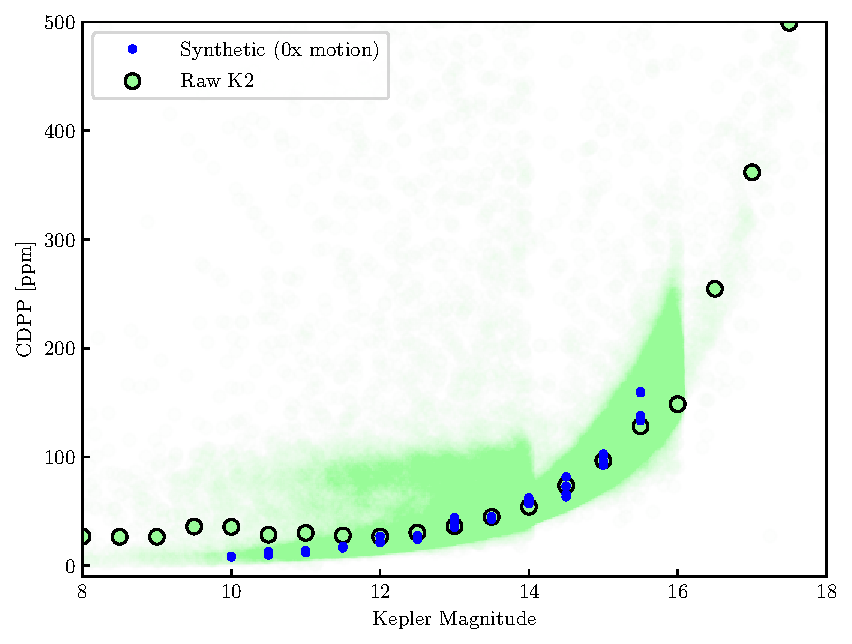
\includegraphics[width=.5\linewidth]{kepler_benchmark.pdf}
	\caption{Photometric precision of our simulated light curves with no motion compared to original \textit{Kepler} targets as a function of $Kp$ Mag. The yellow trend represents the noise as a function of }
	\label{fig:nomotion}
\end{figure}

In our second benchmarking test, we consider the case of current \textit{K2} motion. To do so, we inject motion from 1000 cadences of the \textit{K2} target EPIC 205998445 to benchmark our model against \textit{K2} data. This target is a  \textit{K2} C03 star with $Kp = 12.029$ located near the edge of its detector. Statistics about the motion data used in our simulation can be found in Table \ref{table:motionstatistics}.

\begin{table}[h!]
\begin{center}
    \begin{tabular}{c | c | c}
        Motion Coefficient & Motion (pixels) & Max Motion (pixels) \\
        \hline \hline
        1 & $0.37\pm0.16$ & 0.56 \\
        2 & $0.38\pm0.32$ & 1.12 \\
				5 & $1.04\pm0.75$ & 2.8 \\
				10 & $2.04\pm1.75$ & 6.6 \\
				20 & $3.16\pm1.75$ & 11.2 \\
   \end{tabular}
	 \caption{Motion coefficients and corresponding pixel motion.}
	 \label{table:motionstatistics}
\end{center}
\end{table}

With real \textit{K2} motion applied, sensitivity variation parameters were adjusted until CDPP versus $Kp$ Mag correspended to the trend of real \textit{K2} observations. We found that a stochastic distribution of sensitivity with ${\sim}1\%$ variation between pixels and ${\sim}5\%$ variation within pixels, from center to edge. A sample detector with included sensitivity variation can be seen in Figure \ref{fig:detector_sensitivity}.

\begin{figure}[h]
	\centering
	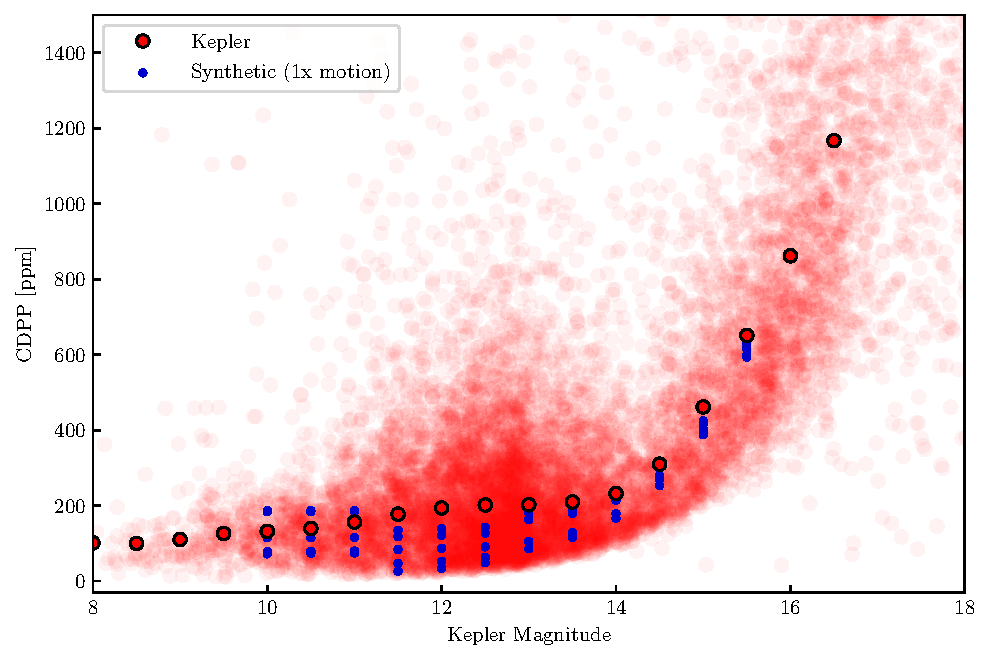
\includegraphics[width=.5\linewidth]{k2_benchmark.pdf}
	\caption{CDPP of our simulated light curves with \textit{K2} motion compared to real \textit{K2} targets as a function of $Kp$ Mag.}
	\label{fig:1motion}
\end{figure}

For campaigns up to 17, stellar PSFs already traverse various regions of sensitivity variation on the CCD due to pointing instability. As spacecraft motion increases, PSFs will move more dramatically across many pixels, which will contribute significant noise to sputtering-\textit{K2} light curves.

\begin{figure}[h]
	\centering
	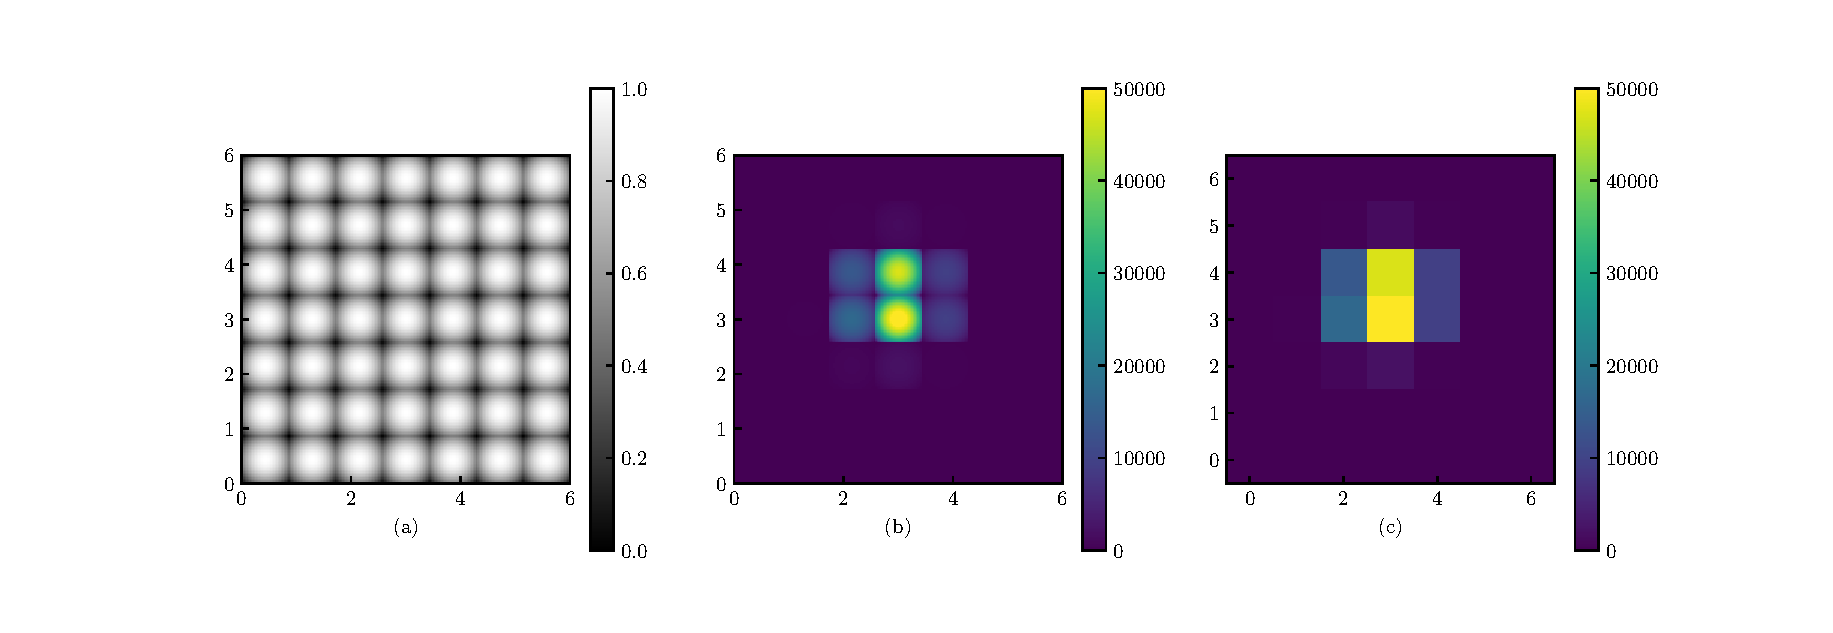
\includegraphics[width=1.0\linewidth]{detector_sensitivity.eps}
	\caption{(a) A sample detector with sensitivity variation, where white represents 100\% photon capture rate, and the shaded regions have lower values for quantum sensitivity. Note that our model peaks in sensitivity at the center of each pixel and falls off towards the edges. There is also random variation in sensitivity between pixels. (b) A Stellar PSF mathematically simulated onto the detector at the sub-pixel level. The sensitivity variation has been exaggerated in this simulation to demonstrate the variation in sub-pixel fluxes. (c) The final interpolated image. The value of each pixel is the integral over $x$ and $y$ of the sub-pixel flux.}
	\label{fig:detector_sensitivity}
\end{figure}

\subsection{High Roll}

To test how PLD performs on targets with high motion relative to the detector, we inject motion vectors with various coefficients into our synthetic models. A coefficient of 1 corresponds to physical \textit{K2} motion (maximum of $\sim 0.56$ pixels), while a coefficient of 20 results in motion of up to $11.2$ pixels.

The resulting raw light curve noise can be seen in Fig. \ref{fig:rawmotion} compared to raw \textit{K2} noise. Our synthetic targets with a motion coefficient of 1 align with the raw \textit{K2} trend and increase corresponding to noise coefficient.

\begin{figure}[h]
	\centering
	\includegraphics[width=1.0\linewidth]{rawmotion.png}
	\caption{CDPP of synthetic targets with 1x to 20x motion versus raw \textit{K2} noise as a function of $K_p\ Mag$.}
	\label{fig:rawmotion}
\end{figure}

\section{Results}

The two sources of noise presented above -- pixel crowding and detector sensitivity variation -- have been obstacles for \textit{K2} de-trending pipelines. In the following section, we present methods to address both sources of noise and recover more accurate light curves.

\subsection{PLD}

After generating a set of light curves representative of extreme motion \textit{K2} observations, we tested systematics removal methods to assess how potentially valuable sputtering-\textit{K2} data would be. To de-trend our synthetic light curves, we used a variant of the method applied in the EPIC Variability Extraction and Removal for Exoplanet Science Targets (\texttt{EVEREST}) pipeline. The \texttt{EVEREST} pipeline utilizes a method called pixel level decorrelation (PLD), developed by \cite{0004-637X-805-2-132} for the \textit{Spitzer} Space Telescope. For a more detailed treatment of PLD, see the first two \texttt{EVEREST} papers \citep{2016AJ....152..100L,2017arXiv170205488L}.

PLD seeks to remove noise generated by intra-pixel sensitivity variation independent of apparent motion of the star. This method is particularly effective for \textit{K2} light curves despite the magnitude of apparent motion being high, and \texttt{EVEREST} can recover \textit{Kepler}-like accuracy in exoplanet light curves for targets up to $\text{Kp} = 15$.

The likelihood ($\mathcal{L}$) of the observed data given our model can be described by a Gaussian distribution given by
%
\[
\mathcal{L} = C * \exp{\left[- \frac{1}{2}\left(\textbf{y} - \textbf{X}\cdot\textbf{w} \right)^\top \cdot \pmb{\Sigma}^{-1} \cdot \left(\textbf{y} - \textbf{X}\cdot\textbf{w} \right) \right]}, \\
\]
%
where $\textbf{y}$ is the raw flux light curve, $\textbf{X}$ is the design matrix constructed from the basis vectors of the intrumental noise in each pixel, $\pmb{\Sigma}$ is the covariance matrix between pixels, $C$ is a normalization constant, and $\textbf{w}$ is the array of weights. By solving for the derivative of the natural log of this likelihood with respect to $\textbf{w}$, we locate the distribution peak and calculate a maximum likelihood estimate of the model parameters.
%
\[
\ln{\mathcal{L}} = - \frac{1}{2}\left(\textbf{y} - \textbf{X}\cdot\textbf{w} \right)^\top \cdot \pmb{\Sigma}^{-1} \cdot \left(\textbf{y} - \textbf{X}\cdot\textbf{w} \right) + C'. \\
\]
%
$C'$ is a constant and becomes $0$ when we differentiate with respect to $\textbf{w}$:
\[
\frac{d\ln{\mathcal{L}}}{d \textbf{w}} = 0 \\
\]
%
\[
\frac{d}{d \textbf{w}} \left[ - \frac{1}{2} \left(\textbf{y} - \textbf{X}\cdot\textbf{w} \right)^\top \cdot \pmb{\Sigma}^{-1} \cdot \left(\textbf{y} - \textbf{X}\cdot\textbf{w} \right) \right] = 0 \\
\]
%
Now, we solve for $\textbf{w}$ to identify the ideal weights for our noise model.
%
\[
\textbf{w} = \left( \textbf{X}^\top \cdot \pmb{\Sigma}^{-1} \cdot \textbf{X} \right)^{-1} \cdot \textbf{X}^\top \cdot \pmb{\Sigma}^{-1} \cdot \textbf{y} \\
\]
%
The final model $\textbf{m}$ can be found by solving $\textbf{m} = \textbf{X} \cdot \textbf{w}$,
%
\[
\textbf{m} = \textbf{X} \cdot \left( \textbf{X}^\top \cdot \pmb{\Sigma}^{-1} \cdot \textbf{X} \right)^{-1} \cdot \textbf{X}^\top \cdot \pmb{\Sigma}^{-1} \cdot \textbf{y}. \\
\]
%

\subsection{Motion Tests}

When de-trended with second order PLD, our synthetic light curves align with the noise of original \textit{Kepler} observations for motion coefficients of 1x, 2x, and 5x. 10x motion shows increased noise in the de-trended light curve, but still performs better than observations from the ground. A detailed look at these results can be found in Fig. \ref{fig:detmotion}.

\begin{figure}[h]
	\centering
	\includegraphics[width=1.0\linewidth]{detmotion.png}
	\caption{De-trended CDPP for synthetic targets with 1x to 20x motion versus original \textit{Kepler} noise as a function of $K_p\ Mag$.}
	\label{fig:detmotion}
\end{figure}


\section{Discussion}

\subsection{Focus Changes}

When \textit{TESS} launches, it will begin observation with a known focusing issue, resulting in larger stellar PSFs. Further, the space telescope's trajectory will cause a periodic variation in the incident sunlight on the telescope, which will affect the quantum sensitivity of pixels. Periodically changing sensitivity will cause \textit{TESS} PSFs to ``breathe" as the temperature rises and falls, and apertures around \textit{TESS} targets will need to expand and contract correspondingly to effectively capture the desired stellar signal.

\section{Using \texttt{scope}}

All of our code is open-source and publically available online. Our simulation package can be installed by running
%
\begin{lstlisting}[language=bash]
git clone https://github.com/nksaunders/scope
cd scope
python setup.py install
\end{lstlisting}
%
To create a light curve with \texttt{scope}, first instantiate a \texttt{Target} object:
%
\begin{lstlisting}[language=Python]
import scope
star = scope.Target()
\end{lstlisting}
%
A light curve can be generated by calling the \texttt{GenerateLightCurve()} function, which returns a light curve of target pixel files (\texttt{fpix}), a one-dimensional flux light curve (\texttt{flux}), and a light curve of the error in each pixel (\texttt{ferr}):
%
\begin{lstlisting}[language=Python]
fpix, flux, ferr = star.GenerateLightCurve()
\end{lstlisting}
%
After a target is created, transits, variability, or neighbors can be added with the following functions:
%
\begin{lstlisting}[language=Python]
star.AddTransit()
star.AddVariability()
star.AddNeighbor()
\end{lstlisting}
Alternatively, the target can be initialized with added features by changing the following boolean parameters:
%
\begin{lstlisting}[language=Python]
star = scope.Target(transit=True, variable=True, neighbor=True)
\end{lstlisting}
%
The detector with sensitivity variation can be displayed by calling
%
\begin{lstlisting}[language=Python]
star.DisplayDetector()
\end{lstlisting}
%
To de-trend with second order PLD, run
\begin{lstlisting}[language=Python]
star.Detrend()
\end{lstlisting}
\section{Conclusions}

We have created a forward model of the \textit{Kepler} space telescope detector, \texttt{skope}, which includes inter- and intra-pixel sensitivity variation and mathematical simulations of stellar PSFs to test de-trending methods for exoplanet targets. Using these simulations, we have demonstrated that \texttt{EVEREST} and PLD are  capable of reducing systematic noise to higher precision than ground based observations in \textit{K2} light curves with up to 10x current spacecraft motion. We have shown that in the event of spacecraft thruster sputtering due to diminishing fuel reserves, valuable data can still be collected and analyzed to benefit \textit{K2} science goals.

Though \textit{TESS}, the successor to \textit{Kepler}, has launched, there remains a wealth of both existing and unobserved \textit{K2} data that offers valuable contribution to our understanding of exoplanetary systems. Earthlike exoplanets can be difficult to identify in the high-magnitude noise of current \textit{K2} data, which will continue to get noisier as the mission reaches its conclusion. The methods we have presented aim to produce the most precise exoplanet identification, characterization, and analysis from the data we have available, and prepare for the next generation of space telescopes.

\textcolor{red}{Acknowledgements.}

This work was supported by NASA grant NNX14AK26G. Computing for this research was performed on the Hyak supercomputer system at the University of Washington.

\clearpage
\bibliographystyle{aasjournal}
\bibliography{references.bib}

\end{document}
